\documentclass[a4paper]{article}
%\usepackage[utf8]{inputenc}
\usepackage[english, swedish]{babel}
\usepackage[T1]{fontenc}

\setlength{\parindent}{0pt}
\setlength{\parskip}{2ex}

%\usepackage[backend=biber, style=apa]{biblatex}
%\usepackage{csquotes}
%\addbibresource{sources.bib}

\usepackage{mathtools}

\usepackage{graphicx}

\usepackage{amsthm} 

\usepackage{amsfonts} 

\usepackage{amssymb}

\usepackage{txfonts}

\usepackage{microtype}

\usepackage{setspace}

\usepackage{hyperref}

\usepackage{hyphsubst}

\usepackage{float}

\usepackage{enumitem}

\usepackage{tikz}

\usepackage{fancyhdr}

\usetikzlibrary{fit, shapes}

\hypersetup{hidelinks}

\usepackage{geometry}
\usepackage{setspace}
\geometry{a4paper,left=60pt,right=60pt,top=60pt, bottom=60pt}
\spacing{1.2}

\makeatletter
\renewcommand*\env@matrix[1][*\c@MaxMatrixCols c]{%
  \hskip -\arraycolsep
  \let\@ifnextchar\new@ifnextchar
  \array{#1}}
\makeatother

\theoremstyle{definition}
\newtheorem{theorem}{Theorem}[section]
\theoremstyle{definition}
\newtheorem{sats}[theorem]{Sats}
\theoremstyle{definition}
\newtheorem{example}[theorem]{Example}
\theoremstyle{definition}
\newtheorem{exempel}[theorem]{Exempel}
\theoremstyle{definition}
\newtheorem{definition}[theorem]{Definition}
\theoremstyle{definition}
\newtheorem{corollary}[theorem]{Corollary}
\theoremstyle{definition}
\newtheorem{korollarium}[theorem]{Korollarium}
\theoremstyle{definition}
\newtheorem{lemma}[theorem]{Lemma}
% \theoremstyle{definition}
% \newtheorem{proof}[theorem]{Proof}
\theoremstyle{definition}
\newtheorem{bevis}[theorem]{Bevis}
\theoremstyle{definition}
\newtheorem{metod}[theorem]{Metod}
\theoremstyle{definition}
\newtheorem{tips}[theorem]{Tips!}
\theoremstyle{definition}
\newtheorem{method}[theorem]{Method}
\theoremstyle{definition}
\newtheorem{problem}[theorem]{Problem}
\theoremstyle{plain}
\newtheorem{obs}[theorem]{OBS!}

\newcommand{\opim}{\operatorname{im}}
\newcommand{\opker}{\operatorname{ker}}
\newcommand{\opspan}{\operatorname{span}}
\newcommand{\opmean}[1]{\overline{#1}}
\newcommand{\opconj}[1]{\overline{#1}}
 


\title{Funktioner och funktionalekvationer}
\author{William Kraft}
\date{\today}


\begin{document}
\pagestyle{fancy}
\fancyhead{}
\fancyhead[L]{\today}
\fancyhead[R]{William Kraft}
\fancyhead[C]{Funktioner och funktionalekvationer}

% \maketitle
% \tableofcontents
% \newpage

\if 0
	TODO!!!
- Ge fler exempel kring tipsen
- Gör första problemen aningen tydligare i vad man förväntas uppnå
\fi



\section{Funktioner}

\begin{definition}[Funktion]
	En funktion är en kartläggning som för varje element i definitionsmängden, ger ett unikt värde i målmängden.
\end{definition}

\begin{exempel}
	Funktionen på bilden har värdet \(1.2\) för invärden \(3\) och 8, och värdet \(0.3\) för invärdet \(-6\).

	\center
	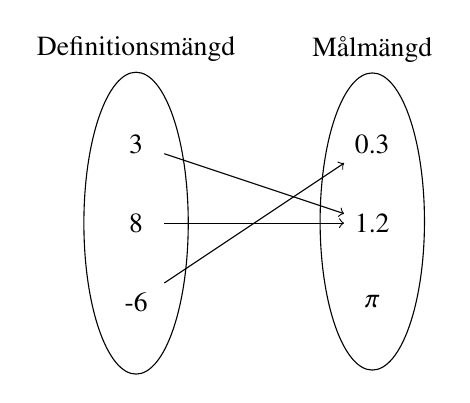
\begin{tikzpicture}
		\begin{scope}[local bounding box=A, x=3cm, y=1cm]
			\node[minimum width=2em] (n-1-A) at (0,-0) {3};
			\node[minimum width=2em] (n-2-A) at (0,-1) {8};
			\node[minimum width=2em] (n-3-A) at (0,-2) {-6};
		\end{scope}
		\node[ellipse, draw, fit=(A), label={above:Definitionsmängd}] {};

		\begin{scope}[local bounding box=B, x=3cm, y=1cm]
			\node[minimum width=2em] (n-1-B) at (1,-0) {0.3};
			\node[minimum width=2em] (n-2-B) at (1,-1) {1.2};
			\node[minimum width=2em] (n-3-B) at (1,-2) {\(\pi\)};
		\end{scope}
		\node[ellipse, draw, fit=(B), label={above:Målmängd}] {};

		\draw[->] (n-1-A) -- (n-2-B);
		\draw[->] (n-2-A) -- (n-2-B);
		\draw[->] (n-3-A) -- (n-1-B);
	\end{tikzpicture}
\end{exempel}

\begin{exempel} \label{exempel:funktioner}
	Det finns många sorters funktioner, både i och utanför matematiken:
	\begin{itemize}
		\item \(f(x) = x^2\)
		\item \(g(n) = \begin{cases} 0, \text{ n udda}  \\ 1, \text{ n jämn} \end{cases}\)
		\item \(u(x, t) = \text{``Värmen i staven \(x\) cm från kanten vid tiden \(t\)''} \) 
		\item \(P(t, p) = \text{``Sannolikheten att tävlande \(t\) i en mattetävling löser problem \(p\) .''} \) 
		\item Funktionen som tar in en funktion, och ger dess invers.
	\end{itemize}
\end{exempel}

\begin{obs}
	Inte alla funktioner behöver vara möjliga att skriva med matematisk notation, eller ens något vi vet hur man beräknar. Men, de måste ge ett och samma svar om de får samma invärden.
\end{obs}


\subsection{Viktiga egenskaper}

\begin{definition}[Injektiv]
	En funktion är injektiv om inga två element i definitionsmängden har samma värde i målmängden.
\end{definition}

\begin{obs}
	Injektiv innebär att om \(f(x) = f(y)\) så måste \(x = y\)
\end{obs}


\begin{definition}[Surjektiv]
	En funktion är surjektiv, om den antar alla värden i målmängden.
\end{definition}

\begin{obs}
	Surjektiv innebär att för varje \(y\), finns ett (eller flera) \(x\) så att \(f(x) = y\).
\end{obs}

\begin{definition}[Inverterbar]
	En funktion är inverterbar om den är både injektiv och surjektiv.
\end{definition}

\begin{definition}[Kontinuerlig (enklare definition)]
	En funktion är kontinuerlig om du kan gå längs grafen över hela definitionsmängden.	
\end{definition}

\begin{obs}
	Exakta definitionen är mer komplicerad, men det här är intuitionen.
\end{obs}

\begin{exempel} Exempel på en surjektiv, injektiv, respektive inverterbar funktion.
	\center
	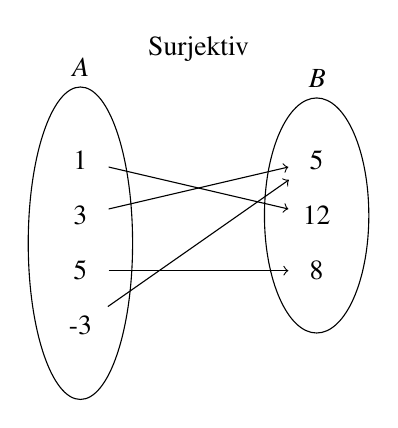
\begin{tikzpicture}
		\foreach[count=\i] \lseti/\lsetmi in {{A}/{1,3,5,-3},{B}/{5,12,8}} {
			\begin{scope}[local bounding box=\lseti, x=3cm, y=0.7cm]
				\foreach[count=\j] \lj in \lsetmi {
					\node[minimum width=2em] (n-\j-\lseti) at (\i,-\j) {\lj};
				}
			\end{scope}
			\node[ellipse, draw, fit=(\lseti), label={above:$\lseti$}] {};
		}
		\draw[->] (n-1-A) -- (n-2-B);
		\draw[->] (n-2-A) -- (n-1-B);
		\draw[->] (n-3-A) -- (n-3-B);
		\draw[->] (n-4-A) -- (n-1-B);
	\node at (current bounding box.north) [] {Surjektiv};
	\end{tikzpicture}
	\hfill
	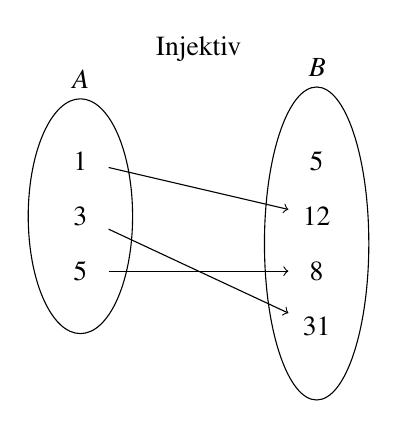
\begin{tikzpicture}
		\foreach[count=\i] \lseti/\lsetmi in {{A}/{1,3,5},{B}/{5,12,8, 31}} {
			\begin{scope}[local bounding box=\lseti, x=3cm, y=0.7cm]
				\foreach[count=\j] \lj in \lsetmi {
					\node[minimum width=2em] (n-\j-\lseti) at (\i,-\j) {\lj};
				}
			\end{scope}
			\node[ellipse, draw, fit=(\lseti), label={above:$\lseti$}] {};
		}
		\draw[->] (n-1-A) -- (n-2-B);
		\draw[->] (n-2-A) -- (n-4-B);
		\draw[->] (n-3-A) -- (n-3-B);
	\node at (current bounding box.north) [] {Injektiv};
	\end{tikzpicture}
	\hfill
	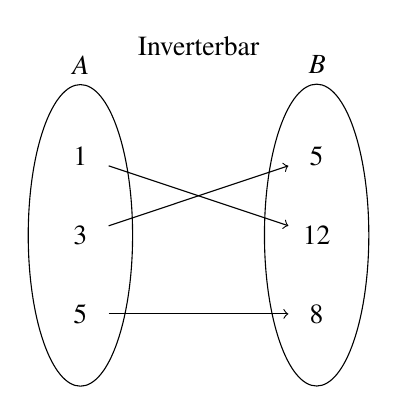
\begin{tikzpicture}
		\foreach[count=\i] \lseti/\lsetmi in {{A}/{1,3,5},{B}/{5,12,8}} {
			\begin{scope}[local bounding box=\lseti, x=3cm, y=1cm]
				\foreach[count=\j] \lj in \lsetmi {
					\node[minimum width=2em] (n-\j-\lseti) at (\i,-\j) {\lj};
				}
			\end{scope}
			\node[ellipse, draw, fit=(\lseti), label={above:$\lseti$}] {};
		}
		\draw[->] (n-1-A) -- (n-2-B);
		\draw[->] (n-2-A) -- (n-1-B);
		\draw[->] (n-3-A) -- (n-3-B);
	\node at (current bounding box.north) [] {Inverterbar};
	\end{tikzpicture}
\end{exempel}

\subsection{Problem}

\begin{problem}
	Vad är definitionsmängden respektive målmängden till funktionerna i exempel \ref{exempel:funktioner}?
\end{problem}

\begin{problem}
	Minska definitionsmängden för \(f(x)=x^2\) så att den blir injektiv. Minska målmängden så att den blir surjektiv. Går det för \(g(x) = 1\)?
\end{problem}

\begin{problem}
	Vilka potensfunktioner, alltså \(f(x) = x^n\) där \(n\) är ett positivt heltal, är surjektiva? Injektiva?
\end{problem}

\begin{problem}
	Hitta en inverterbar funktion från \((0, 1)\), intervallet mellan \(0\) och \(1\), till reella talen.
\end{problem}

\begin{problem}
	Hitta inversen till:
	\begin{itemize}
		\item \(f(x) = x^3\) 
		\item \(f(x) = \sqrt{3x - 1}\) 
		\item \(f(x) = \begin{cases} x^3, & x < 0 \\ \sqrt{3x-1}, &x \geq 1  \end{cases} \)  % TODO Skapa en svår!
	\end{itemize}
\end{problem}

\begin{problem}
	Är en injektiv funktion av en injektiv funktion injektiv? Är en surjektiv funktion av en surjektiv funktion surjektiv?
\end{problem}

\begin{problem}
	Låt \(f(x)\) vara injektiv men inte surjektiv, och \(g(x)\) vara surjektiv men inte injektiv. 
	\begin{enumerate}[label={\alph*)}]
		\item Kan \(h(x) = g(f(x))\) vara inverterbar? Ge ett exempel eller motbevisa.
		\item Vad gäller för \(k(x) = f(g(x))\)?
	\end{enumerate}
\end{problem}

\begin{problem}
	Varför är en funktion inverterbar om den är både surjektiv och injektiv? Varför räcker det inte med ena?
\end{problem}

\begin{problem}
	Låt \(f(x) = x^2\) vara en injektiv funktion med värdemängd alla \textbf{positiva} reella tal. Beskriv alla möjliga definitionsmängder! (Definitionsmängden behöver inte vara sammanhängande)
\end{problem}

\begin{problem}
	Hur ser grafen till en kontinuerlig injektiv funktion ut? Vad utmärker dem? Prata med en kamrat! Vad händer om den dessutom är surjektiv?
\end{problem}

\begin{problem}
	Visa att \(f(x) = \sum_{k=0} ^{101} (-x)^k\) är surjektiv! (Tips! Använd att den är kontinuerlig)
\end{problem}

\begin{problem}
	Visa att \(f(x) = \sum_{k=0} ^{100} (-x)^k\) inte är surjektiv! (Tips! Använd att den är kontinuerlig)
\end{problem}

\begin{problem}
	Visa att funktionen
	\[
		f(x) = x^{101} - \frac{1}{x} + 2^{x^2 + 2}
	\]
	definierad på de \textbf{positiva} reella talen, är inverterbar. (Tips! Rita den!)
\end{problem}

\begin{problem}
	Låt \(f(x)\) vara en funktion från talen \(1,\dots, n\), till talen \(1, \dots ,n\). Varför är den surjektiv om och endast om den är injektiv?
\end{problem}



%   - Finns det ett värde som får denna? (För olika funktioner)
%   - Surjektiv, injektiv, på diskret mapping?
%   - Varför är första ok, men inte den andra?
%     - Funktioner som går in i varandra så att värdemängd ej matchar 
%     - Funktioner som går in i varandra så att värdemängd matchar 
%   - Surjektiv på surjektiv, är den surjektiv? Injektiv?
%   - Injektiv på injektiv, är den surjektiv? Injektiv?
%   - Injektiv, surjektiv på begränsade intervall?
%   - Bestäm värdemängd av klurigt tudelat problem
%   - Bestäm invers
%   - Visa att det finns en invers






\section{Funktionalekvationer}

Ibland får man inte givet vad en funktion är, utom måste lista ut det! Det sker ofta i formen av funktionalekvationer. Stort tack till Neo Dahlfors, vars motsvarande lektion i funktionalekvationer varit stommen för denna.

\begin{exempel}
	Ett exempel på en funktionalekvation är att
	\[
		(x,y): f(x) + f(y) = x + y
	\]
	\textbf{för alla} värden på \(x, y\). Vi försöker alltså inte hitta värden på \(x, y\) som i en vanlig ekvation, utom vet att det gäller för alla, och vill hitta funktionen! 
	I den här funktionalekvationen, kan vi sätta in \(x=z, y=-z\) (eftersom vi får välja fritt bland \(x, y\)), och får
	\[
		(z, -z) : f(z) + f(z) = z + z \Rightarrow f(z) = z.
	\]
\end{exempel}

\subsection{Tips!} % TODO! Utveckla
\begin{tips}[Substitution]
	Sätt in värden på parametrarna som ger bättre samband. Det är ofta bra att pröva \(\left(x, x\right)\), \((x, -x)\), \((0, 0)\), \((x, 0)\) och \((0, y)\) 
\end{tips}

\begin{tips}[Symmetri]
	Sätt in värden på parametrarna som gör om ena delen av ekvationen lik en annan.
\end{tips}

\begin{tips}[Bestäm \(f(0)\)]
	Bestäm (om möjligt) värdet på \(f(0)\), och använd det för att bestämma hur funktionen ändras.
\end{tips}

\begin{tips}
	Utnyttja injektivitet! Injektivitet gör att du kan ``skala bort'' funktionen, alltså att \(f(x) = f(x)\) ger \(x = y\).
\end{tips}

\begin{tips}
	Utnyttja surjektivitet! Surjektivitet gör att du kan substituera in funktionen, ty du vet att det finns ett invärde \(\alpha \), så att \(f(\alpha ) = x\).
\end{tips}

\begin{tips}
	Skapa en ny funktion, definierad från den givna, som är enklare att hantera.
\end{tips}


\subsection{Problem}
\begin{problem}
	Bestäm \(f(x) : \mathbb{R} \rightarrow \mathbb{R} \) om
	\[
		2f(x) - f(-x) = x
	\]
\end{problem}
\begin{problem}
	Finn alla funktioner \(f: \mathbb{R} \rightarrow \mathbb{R} \) sådana att
	\[
		2 f(x) + f(1-x) = 2x + 5
	\]
\end{problem}


\begin{problem}
	Låt 
	\[
		f(x^2+ f(y)) = y + f(x^2).
	\]
	Visa att \(f(x)\) är surjektiv! Visa att den är injektiv!
\end{problem}


\begin{problem}[SMT kval 2007]
	Vilka funktioner \(f(x)\) uppfyller likheten
	\[
		x(f(X) + f(-x) + 2) + 2f(-x) = 0
	\]
\end{problem}

\begin{problem}[SMT final 2008]
	Funktionen \(f(x)\) har egenskapen att \(\frac{f(x)}{x} \) är växande för \(x>0\). Visa att (för alla \(x, y > 0\))
	\[
		f(x) + f(y) \leq f(x+y).
	\]
\end{problem}

\begin{problem}[SMT final 2014]
	Bestäm alla funktioner \(f: \mathbb{R} \rightarrow \mathbb{R} \) sådana att (för alla reella tal \(x, y\))
	\[
		f(f(x+y) - f(x-y)) = xy.
	\]
\end{problem}


%\printbibliography[heading=bibintoc,title=References,]
\end{document}
